\documentclass[12pt,letterpaper]{article}

\usepackage[utf8]{inputenc}

% Page layout
%\usepackage[a4paper]{geometry}
%\geometry{hscale=0.75,vscale=0.75,centering}
\usepackage{fullpage}

% Include images
\usepackage{graphicx}

% Math equations
\usepackage{amsmath}
\usepackage{amssymb}
\usepackage[french]{babel}

% Include Matlab code with accents
\usepackage{listingsutf8}
\lstset{inputencoding=utf8/latin1}
\usepackage[framed]{mcode}


\begin{document}

    \begin{titlepage}
    \vspace*{3.5cm}
    \begin{center} 
        \LARGE{ \textbf{IFT6095 - Sujets en infographie} }\\[1cm]
        \Large{Travail pratique numéro 1.}\\
        \normalsize{20/01/2014}\\[1cm]
        \normalsize{ \textit{Anis Benyoub} }
    	\begin{figure}[ht]
	\centering
	\end{figure}
    \end{center}
    
\end{titlepage}
     
	\newpage 
    
    \section{Rastérisation et shaders programmables:}
	\setlength{\parindent}{1cm}

    Je n'ai pas utilisé de librairies externes (mis à part glMatrix pour la gestion des matrices) pour construire mon programme. Voici le rendu final demandé pour cette partie:\\
\begin{figure}[h!]
	\centering
	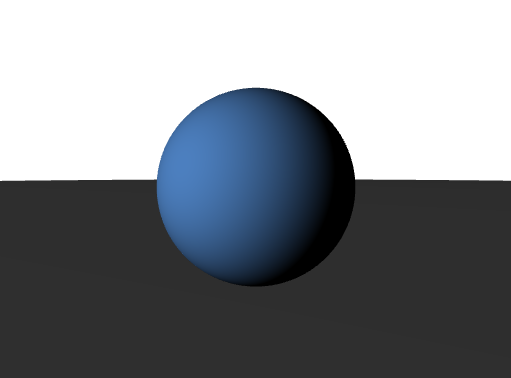
\includegraphics[scale=0.4]{images/rast.png}
	\caption{\textit{Rendu de la scene par rastérisation}}
\end{figure}

	L'utilisation du modèle de shading GL\_SMOOTH permet d'activer l'interpolation des valeurs de type varying lors de la rasterisation par la pipeline OpenGL. Si nous desactivons cette interpolation par l'activation de l'option de shading GL\_FLAT nous perdons donc cette interpolation. Nous pourrions comparer ce changement à la différence entre le modèle d'illumination par sommet (GOURAUD) à celui par fragment (PHONG).\\\\
	Si on élève suffisament le taux de tesselation on peut arriver au cas où la taille d'une primitive (triangle dans notre cas) est plus petite ou égale à un fragment et dans ce cas ces deux modèles deviennent extrèmement semblables.\\\\

	Voici quelques images illustrant l'apport de la tesselation au modèle d'illumination:\\
	\newpage

\begin{figure}[h!]
	\centering
	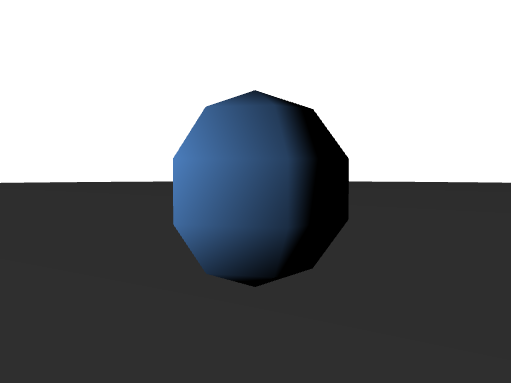
\includegraphics[scale=0.3]{images/tess1.png}
	\caption{\textit{Facteur de tesselation 5}}
	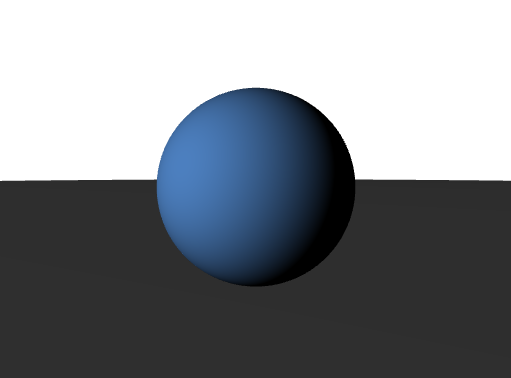
\includegraphics[scale=0.3]{images/rast.png}
	\caption{\textit{Facteur de tesselation 100}}
\end{figure}

	Malheuresement la version 2.0 d'OpenGL ES ne prévoit pas la fonction glShadeModel, je ne peux donc pas produire de screenshot sans écrire une illumination par sommets.\\

    \section{Lancer de rayons avec Javascript sur le CPU}

    Voici le rendu final demandé pour cette partie:

\begin{figure}[h!]
	\centering
	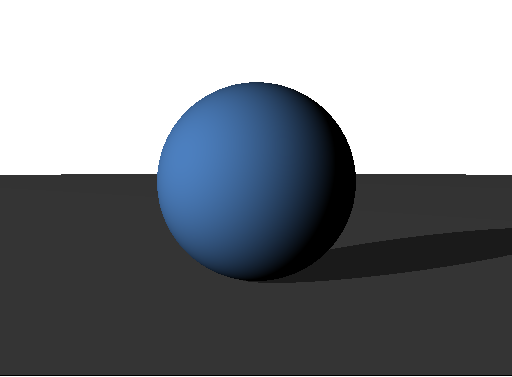
\includegraphics[scale=0.3]{images/ray.png}
	\caption{\textit{Rendu de la scene par lancer de rayon avec rayon secondaire.}}
\end{figure}
    \section{Bonus:}

	\setlength{\parindent}{1cm}
	J'ai décidé d'implémenter dans le lanceur de rayon l'intersection avec les triangle et ce de manière optimisée (basé sur l'article de recherche mentionné dans le code), ainsi que les rayons réfléchi et réfractés. Une notion d'energie de rayon a été introduite pour limiter les niveaux de recursivité.\\\\
	J'ai aussi introduit une illumination ponctuelle pour avoir un rendu plus réaliste.\\
	Voici le resultat graphique obtenu:\\
\begin{figure}[h!]
	\centering
	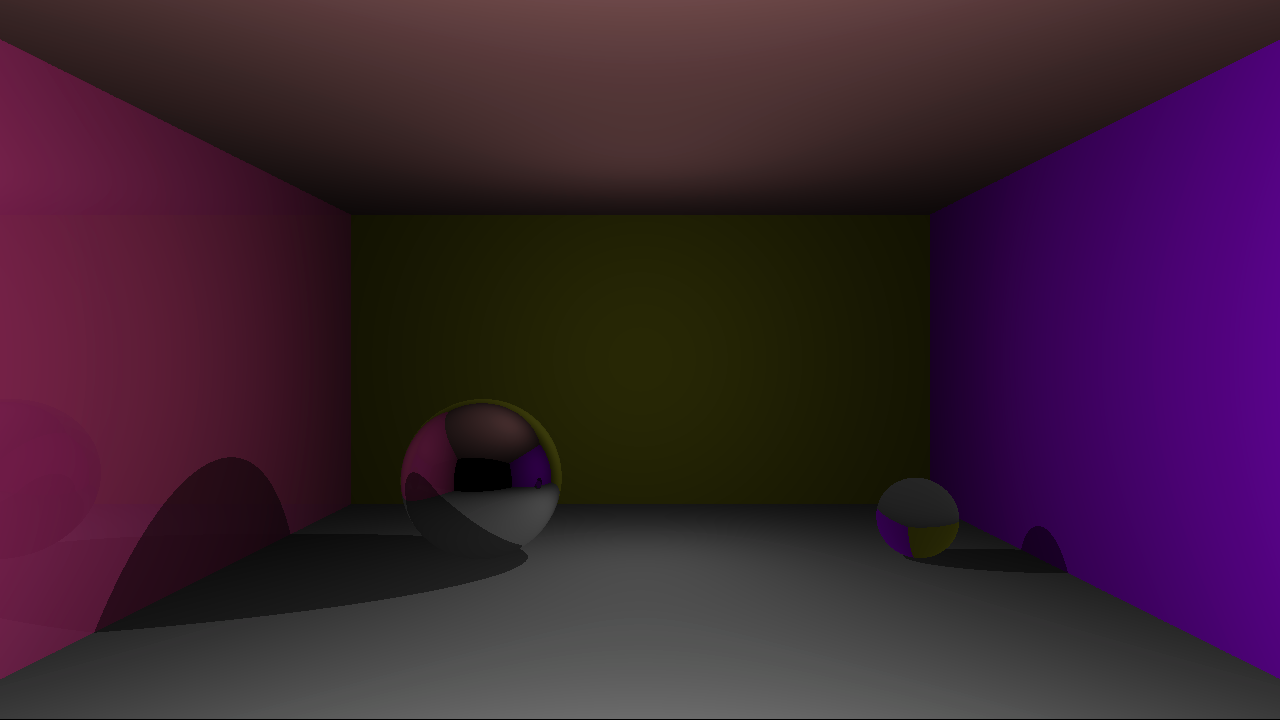
\includegraphics[scale=0.3]{images/extra.png}
	\caption{\textit{Rendu de la partie Bonus}}
\end{figure}

\newpage
    
\end{document}

